\chapter{Anhang}

\begin{figure}[H]
\raggedright
\caption{Verwendete Ressourcen}
\label{Abb:Ressourcen}
\textbf{Hardware:}
\begin{itemize}
\item Büroarbeitsplatz mit Standrechner
\end{itemize}
\textbf{Software:}
\begin{itemize}
\item Windows 7 Professional Service Pack 1 - Betriebssystem
\item Unity 3D Version 5.3.3f1 - 3D Entwicklungsumgebung
\item Visual Studio 2015 - Code Entwicklungsumgebung
\item MiK\TeX - Distribution des Textsatzsystems \TeX
\item \TeX{}Maker - \LaTeX Schreibprogramm
\item Dia Version 0.97.2 - Anwendung zum Zeichnen strukturierter Diagramme
\end{itemize}
\begin{itemize}
\item Entwickler - Implementierung der Scripte / Realisierung
\item Anwendungsentwickler - Code Begutachtung
\end{itemize}
\end{figure}

\begin{figure}[H]
\centering
\caption{Model View Controller}
\label{Abb:MVC}
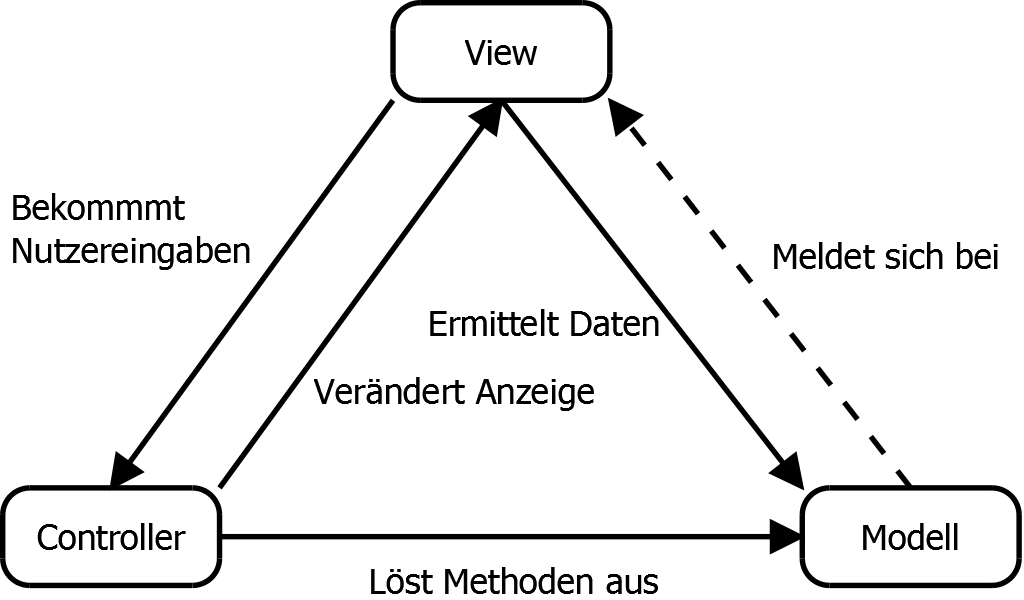
\includegraphics[scale=0.5]{Bilder/Diagramme/MVC.png}
\end{figure}

\begin{figure}[H]
\centering
\caption{Presentation Abstraction Control}
\label{Abb:PAC}
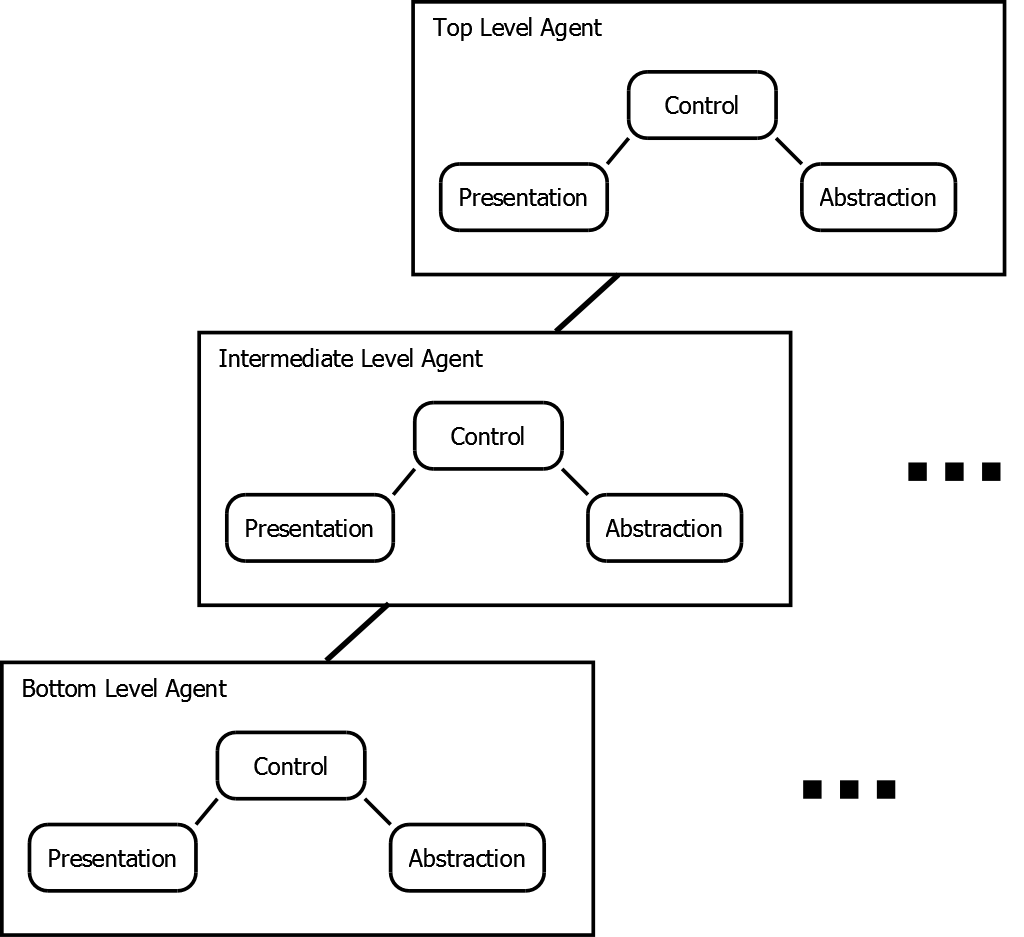
\includegraphics[scale=0.275]{Bilder/Diagramme/PAC.png}
\end{figure}

\begin{figure}[H]
\centering
\caption{Benutzer Oberfläche Skizze}
\label{Abb:UISkizze}
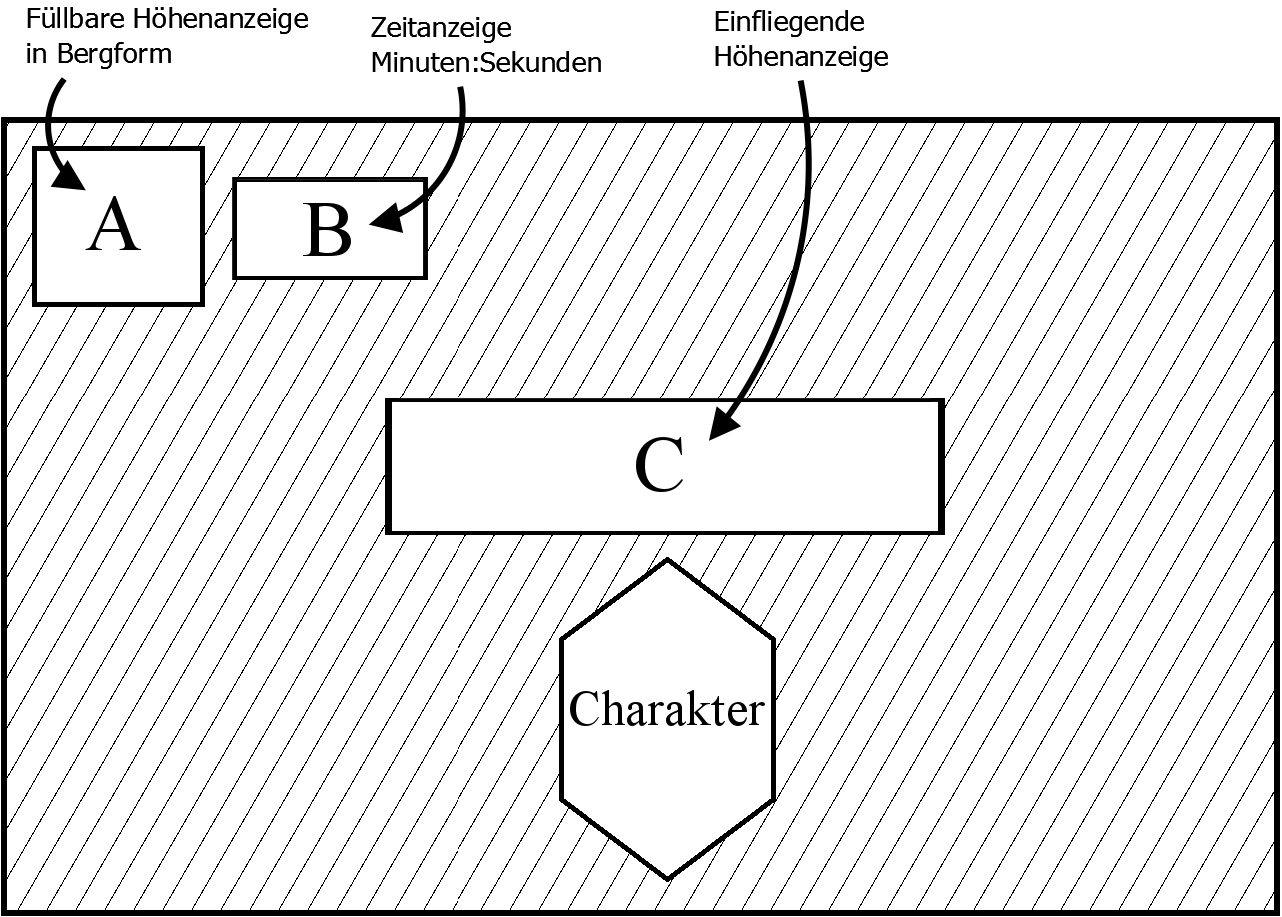
\includegraphics[scale=0.285]{Bilder/Diagramme/UserInterface.png}
\end{figure}

\begin{figure}[H]
\centering
\caption{Benutzer Oberfläche Im Spiel}
\label{Abb:UIIngame}
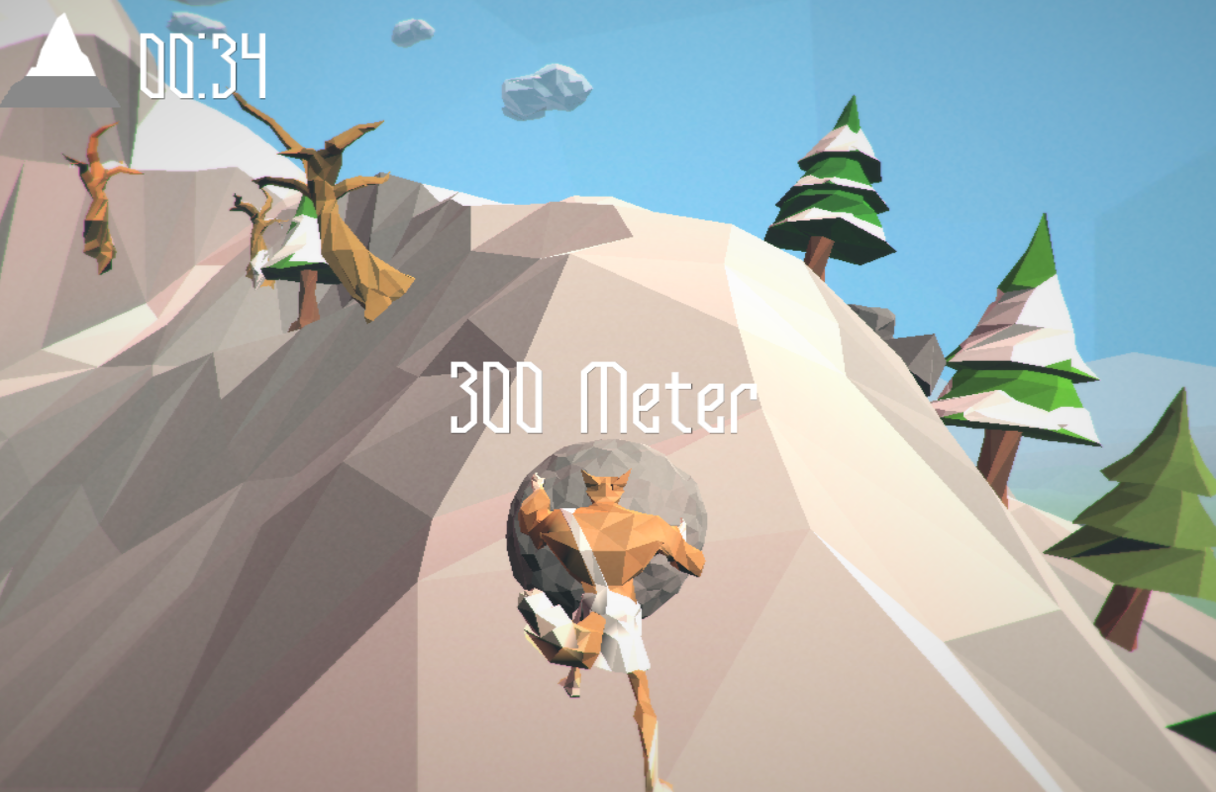
\includegraphics[scale=5.25]{Bilder/SisyfoxUI.png}
\end{figure}

\begin{figure}[H]
\centering
\caption{Klassendiagramm Charaktersteuerung mit Sphere}
\label{Abb:KlassendiaMain}
%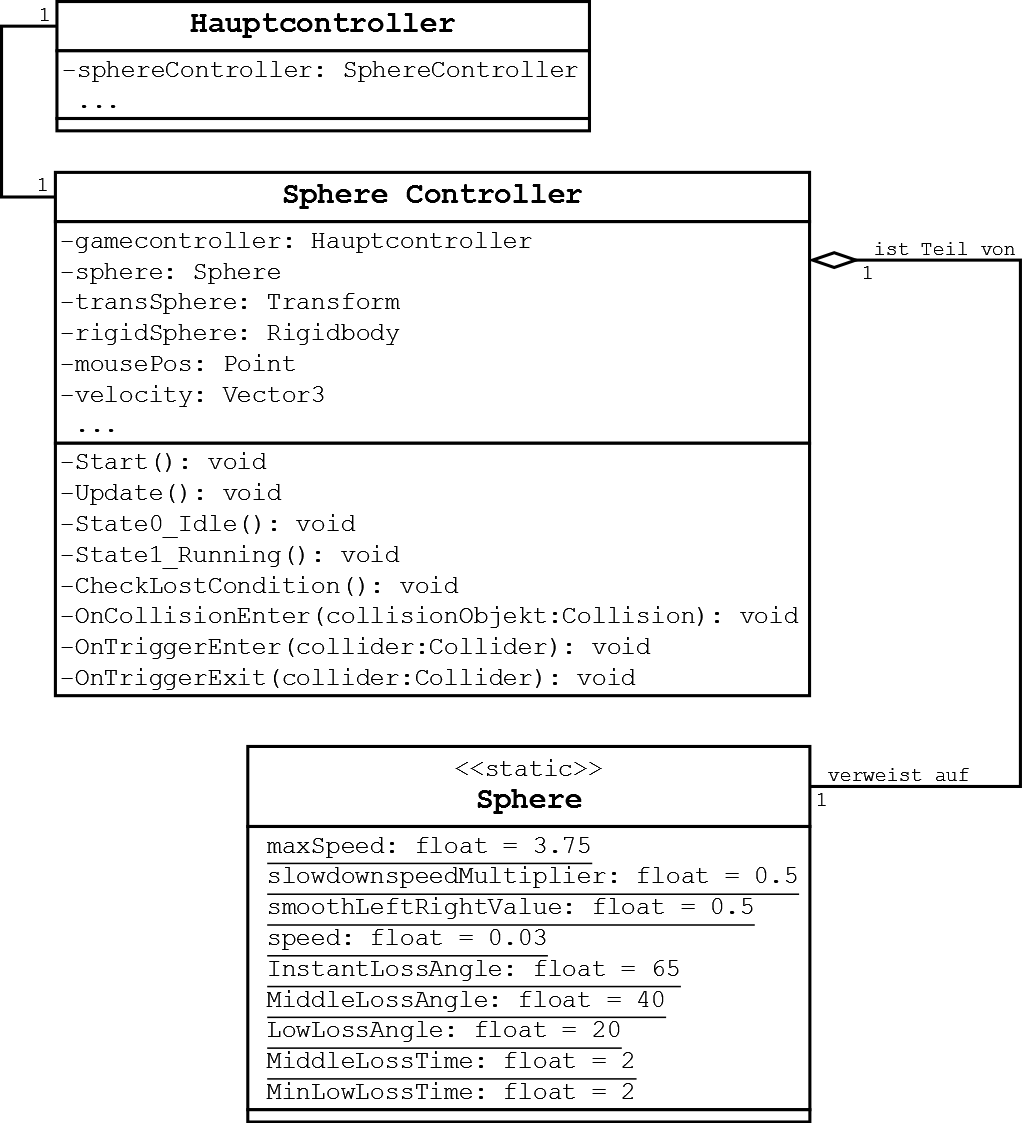
\includegraphics[scale=0.3]{Bilder/Diagramme/KlassendiagrammMain.png}
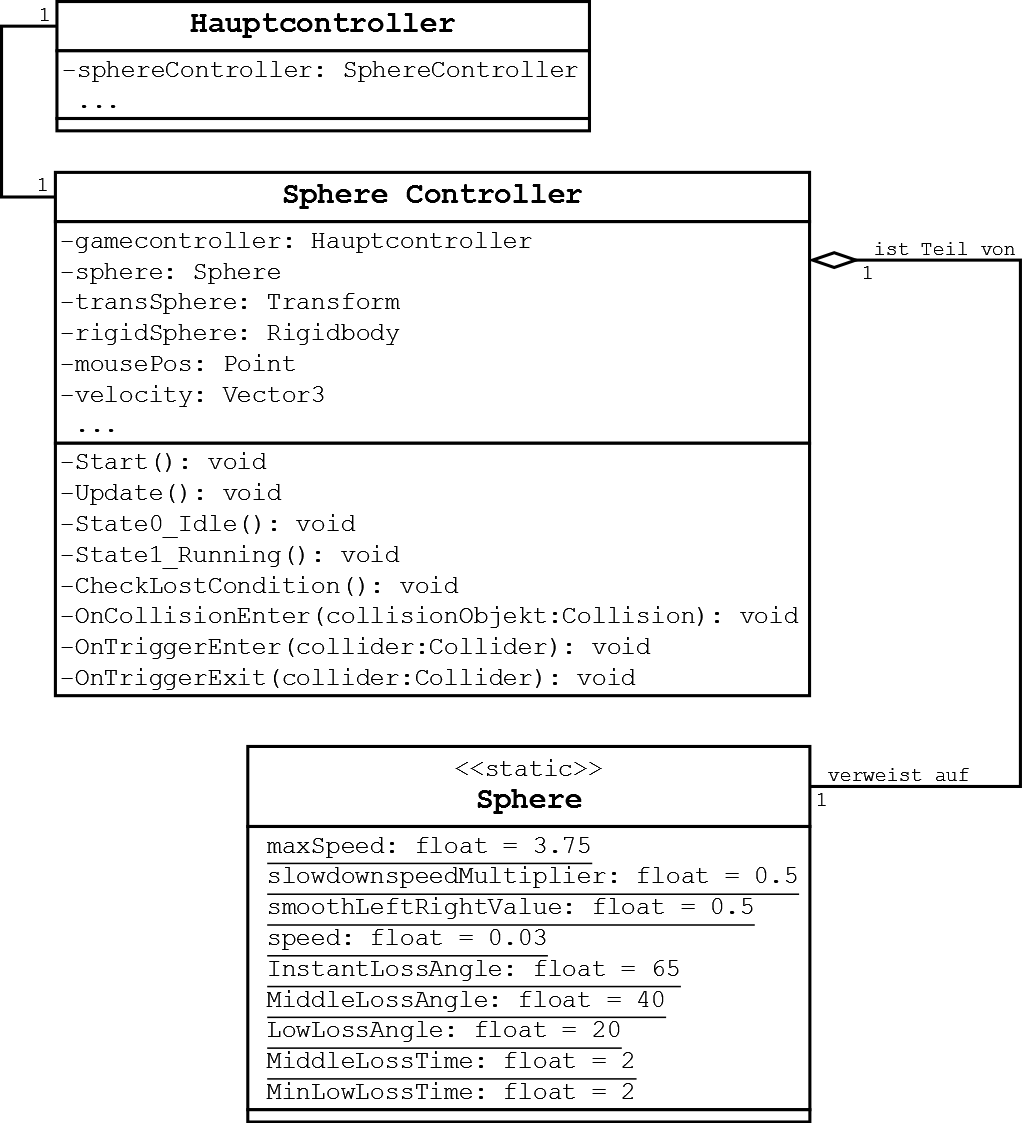
\includegraphics[width=\textwidth, height=0.6\textwidth]{Bilder/Diagramme/KlassendiagrammMain.png}
\end{figure}

\begin{figure}[H]
\centering
\caption{Zustandsdiagramm Statusverwaltung}
\label{Abb:SMStatus}
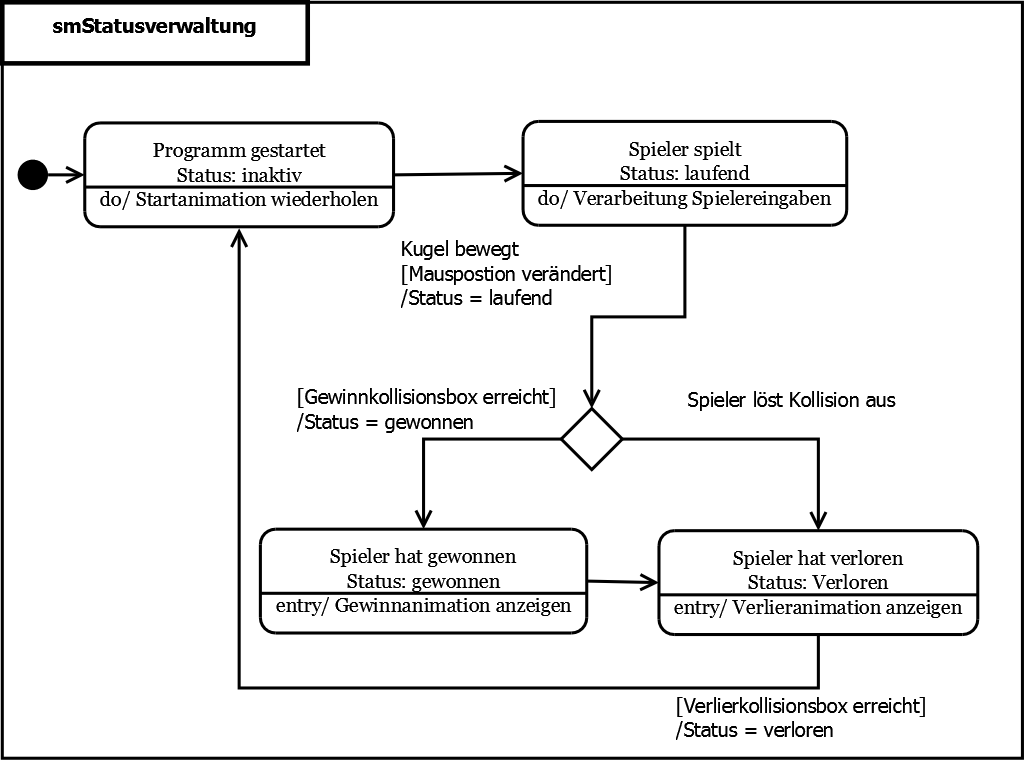
\includegraphics[scale=0.425]{Bilder/Diagramme/smStatusverwaltung.png}
\end{figure}

\begin{figure}[H]
\centering
\caption{Gewinn Triggerbox am Gipfel des Berges}
\label{Abb:GewinnTrigger}
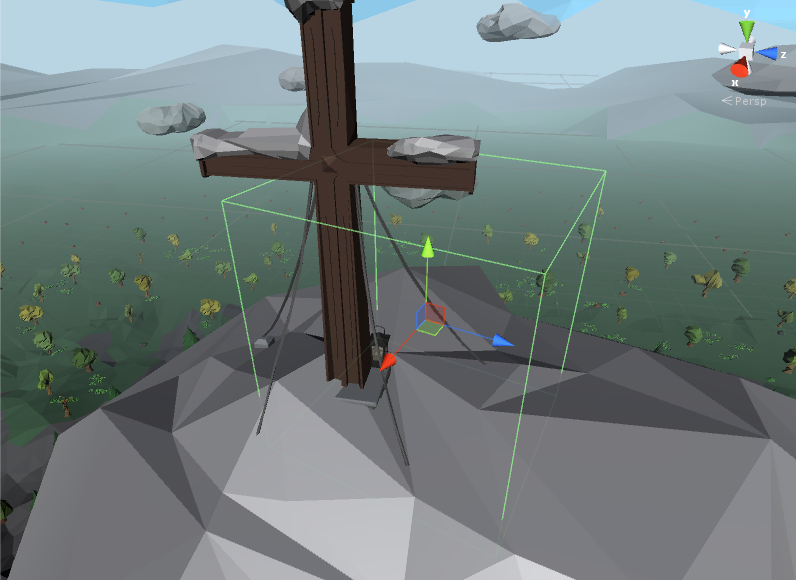
\includegraphics[scale=0.55]{Bilder/GewinnTrigger.png}
\end{figure}

\begin{figure}[H]
\centering
\caption{Baum Triggerbox}
\label{Abb:BaumTrigger}
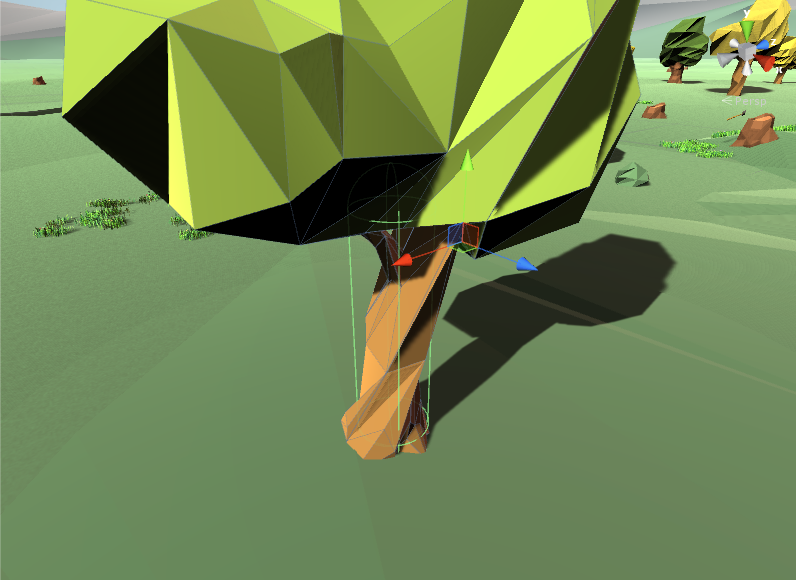
\includegraphics[scale=0.55]{Bilder/BaumTrigger.png}
\end{figure}

\begin{figure}[H]
\centering
\caption{Verloren Status bei seitlichem Steigungswinkel}
\label{Abb:SeitlWinkel}
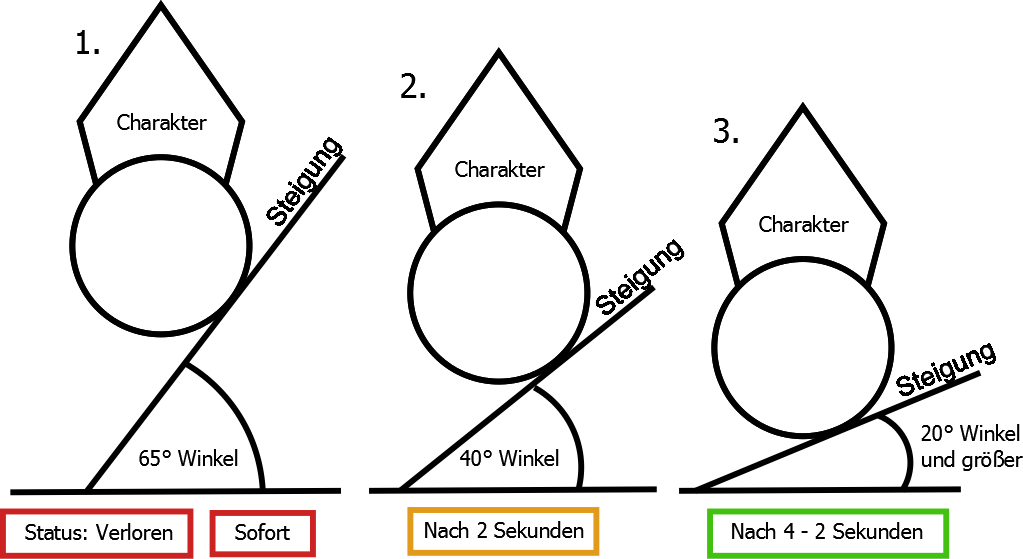
\includegraphics[scale=0.275]{Bilder/Diagramme/VerlierWinkelSeitlich.png}
\end{figure}

\begin{figure}[H]
\centering
\caption{Busch Triggerbox am Rand des Berges}
\label{Abb:BuschTrigger}
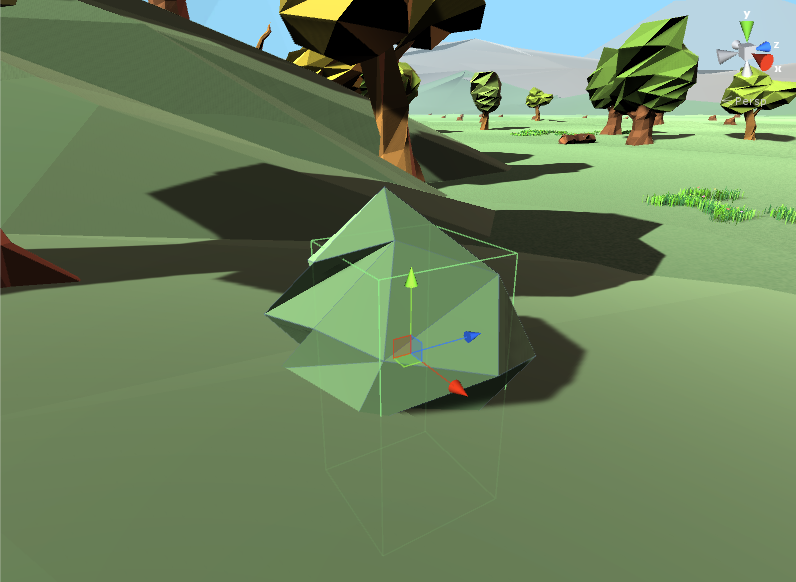
\includegraphics[scale=0.55]{Bilder/BuschTrigger.png}
\end{figure}

